% En este apendice incluimos imágenes de mayor tamaño que no caben en el cuerpo del documento.

Este apéndice contiene imágenes de mayor tamaño que no caben en el cuerpo del documento. Algunas imágenes son versiones ampliadas de las imágenes que se han mostrado en el cuerpo del documento, otras son imágenes adicionales que no se han mostrado en el cuerpo del documento. En la tabla \ref{tab:larger_images} se puede ver una lista de las imágenes que se van a mostrar en este apéndice.

% Tabla indicando las imágenes adicionales que se van a mostrar en este apéndice
\begin{table}[H]
    \centering
    \begin{tabular}{|c|c|}
        \hline
        \textbf{Imagen} & \textbf{Descripción} \\ \hline
        \ref{fig:example_damage_types_large} & Ejemplos de los tipos de daños en el pavimento de la CRDDC2022. \\ \hline
        \ref{fig:example_images_region_large} & Ejemplos de imágenes de los datos de la CRDDC2022. \\ \hline
    \end{tabular}
    \caption{Imágenes adicionales mostradas en este apéndice.}
    \label{tab:larger_images}
\end{table}

% Añadimos img/example_damage_types_grid.png en tamaño grande ocupando toda la página en horizontal
\begin{figure}[H]
    \centering
    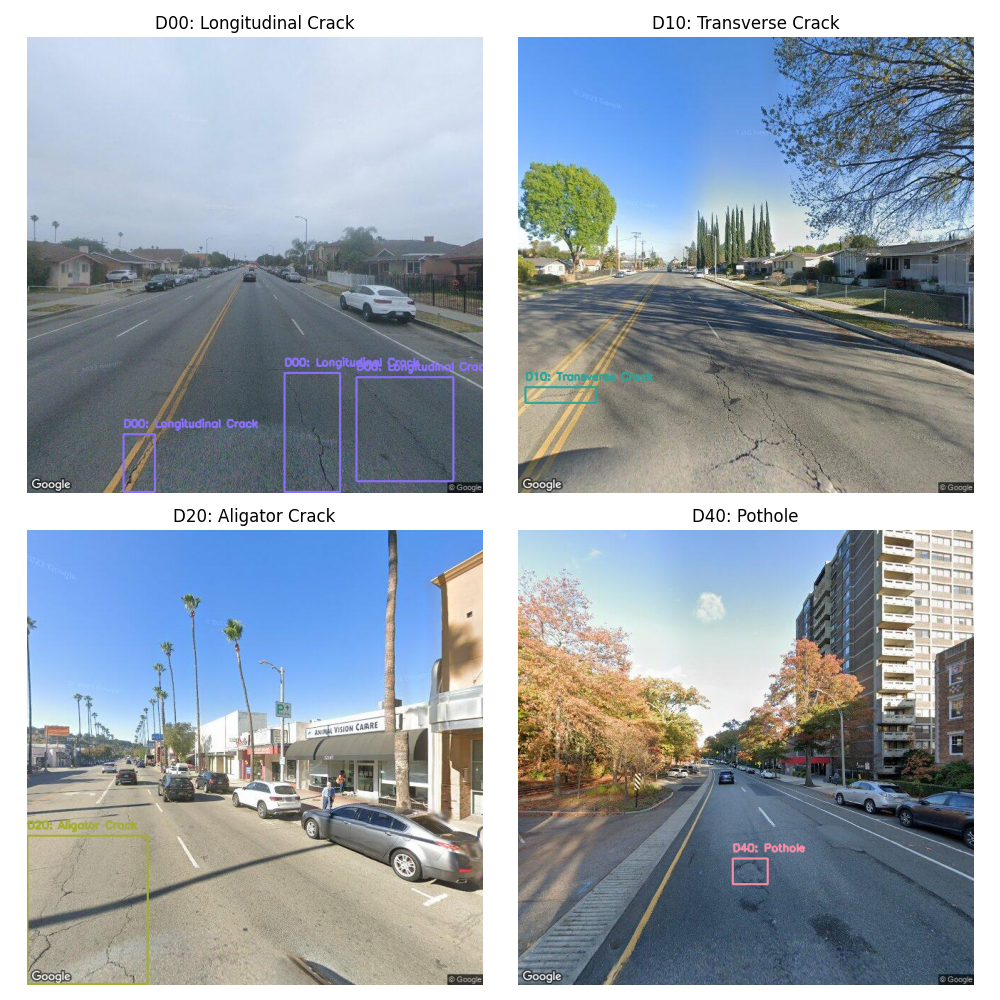
\includegraphics[width=\textwidth,height=\textheight,keepaspectratio]{img/example_damage_types_grid.png}
    \caption{Ejemplos de los tipos de daños en el pavimento de la CRDDC2022. Solo se han marcado los daños en el pavimento correspondientes a la clase que se quiere mostrar.}
    \label{fig:example_damage_types_large}
\end{figure}

% Añadimos img/example_images_regions.png en tamaño grande ocupando toda la página en vertical
\begin{sidewaysfigure}
    \centering
    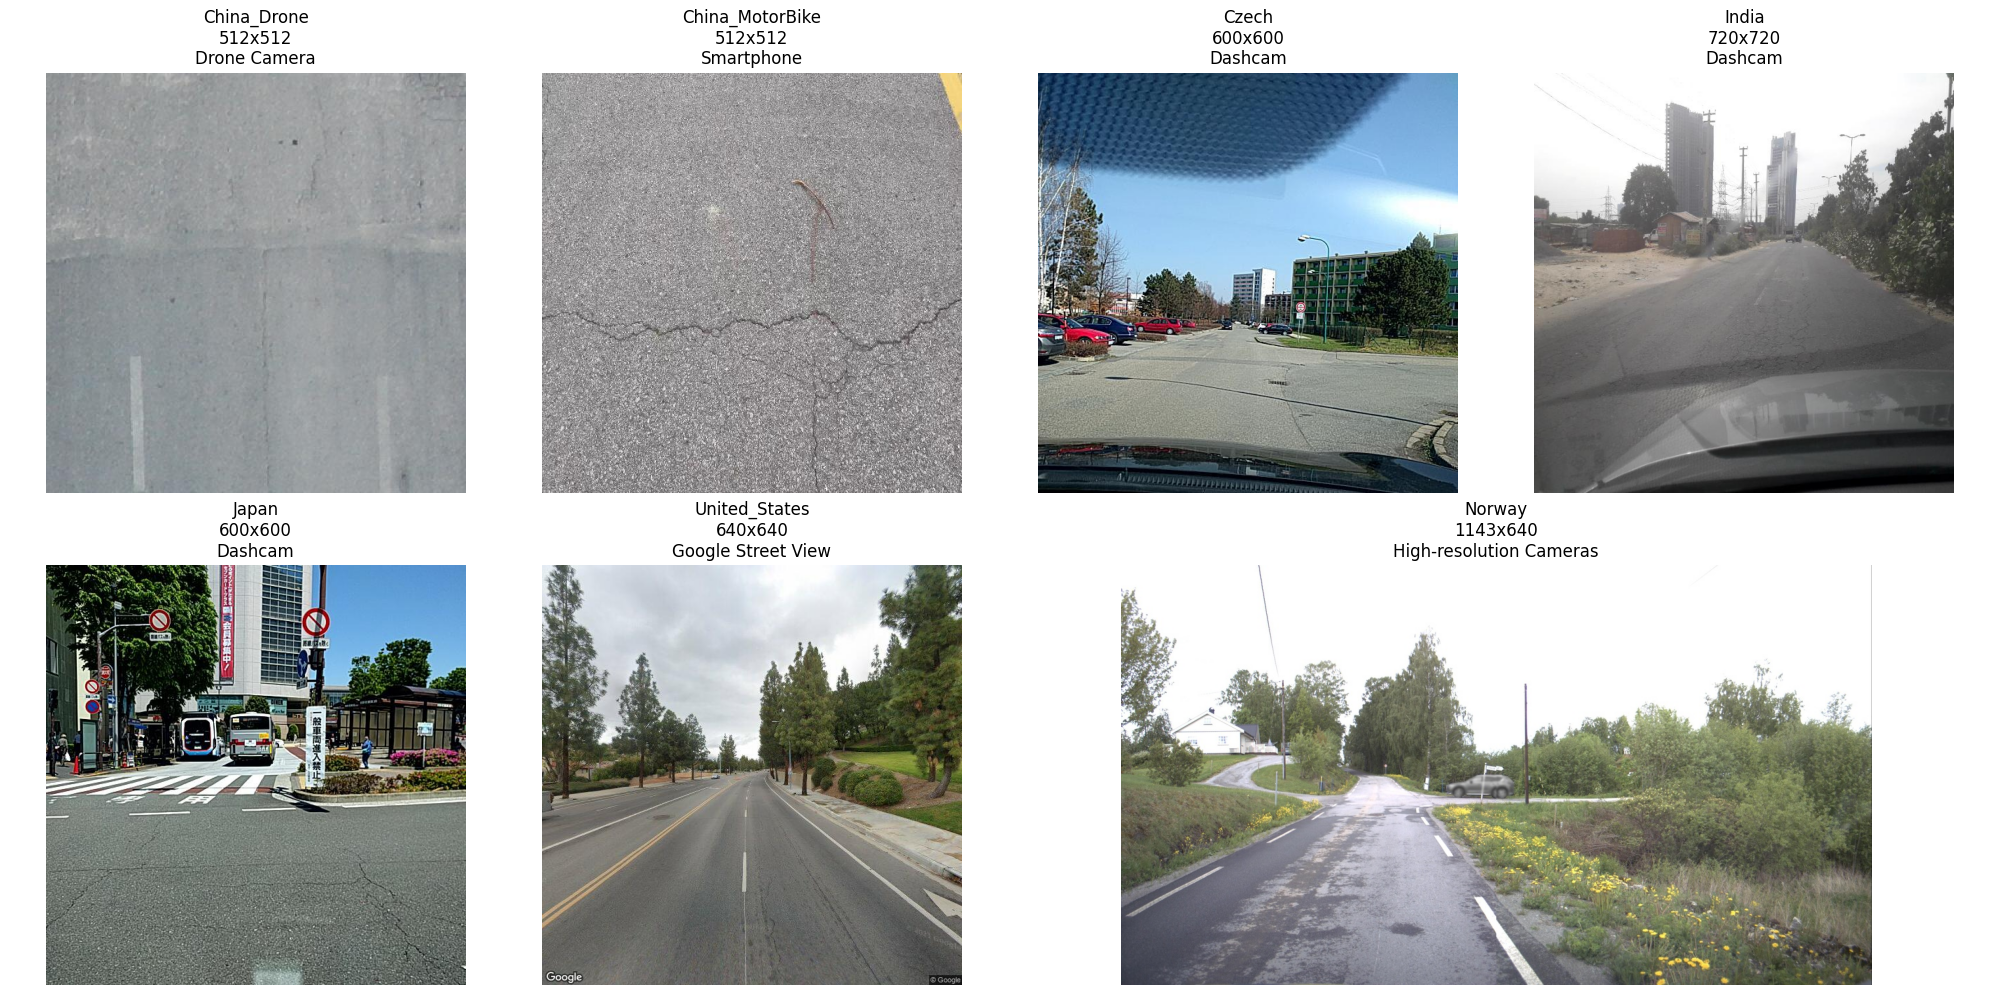
\includegraphics[height=\textheight,width=\textwidth,keepaspectratio]{img/example_images_regions.png}
    \caption{Ejemplos de imágenes de los datos de la CRDDC2022.}
    \label{fig:example_images_region_large}
\end{sidewaysfigure}